% Institute of Computer Science thesis template
% authors: Sven Laur, Liina Kamm
% last change Tõnu Tamme 03.05.2019
%--
% Compilation instructions:
% 1. Choose main language on line 55-56 (English or Estonian)
% 2. Compile 1-3 times to get refences right
% pdflatex bachelors-thesis-template
% bibtex bachelors-thesis-template
%--
% Please use references like this:
% <text> <non-breaking-space> <cite/ref-command> <punctuation>
% This is an example~\cite{example}.

\documentclass[12pt]{article}

% A package for setting layout and margins for your thesis
\usepackage[a4paper]{geometry}
\usepackage{pdflscape}

%%=== A4 page setup ===
%\setlength{\paperwidth}{21.0cm}
%\setlength{\paperheight}{29.7cm}
%\setlength{\textwidth}{16cm}
%\setlength{\textheight}{25cm}


% When you write in Estonian then you want to use text with right character set
% By default LaTeX does not know what to do with õäöu letters. You have to specify
% a correct input and font encoding. For that you have to Google the Web
%
% For TexShop under MacOS X. The right lines are
%\usepackage[applemac]{inputenc}
%\usepackage[T1]{fontenc} %Absolutely critical for *hyphenation* of words with non-ASCII letters.
%
% For Windows and Linux the right magic lines are
% \usepackage[latin1]{inputenc}
% \usepackage[latin5]{inputenc}
%
\usepackage[utf8]{inputenc} %standard encoding since 2018 (can be commented out?)
\usepackage[T1]{fontenc} %Absolutely critical for *hyphenation* of words with non-ASCII letters.

% Typeset text in Times Roman instead of Computer Modern (EC)
\usepackage{times}

% Suggested packages:
\usepackage{microtype}  %towards typographic perfection...
\usepackage{inconsolata} %nicer font for code listings. (Use \ttfamily for lstinline bastype)

\usepackage[section]{placeins}

% Use package babel for English or Estonian
% If you use Estonian make sure that Estonian hyphenation is installed
% - hypen-estonian or eehyp packages
%
%===Choose the main language in thesis
\usepackage[estonian, english]{babel} %the thesis is in English
%\usepackage[english, estonian]{babel} %the thesis is in Estonian


% Change Babel document elements
\addto\captionsestonian{%
    \renewcommand{\refname}{Viidatud kirjandus}%
    \renewcommand{\appendixname}{Lisad}%
}


% If you have problems with Estonian keywords in the bibliography
%\usepackage{biblatex}
%\usepackage[backend=biber]{biblatex}
%\usepackage[style=alphabetic]{biblatex}
%% plain --> \usepackage[style=numeric]{biblatex}
%% abbrv --> \usepackage[style=numeric,firstinits=true]{biblatex}
%% unsrt --> \usepackage[style=numeric,sorting=none]{biblatex}
%% alpha --> \usepackage[style=alphabetic]{biblatex}
%\DefineBibliographyStrings{estonian}{and={ja}}
%\addbibresource{masters-thesis-template.bib}


% General packages for math in general, theorems and symbols
% Read ftp://ftp.ams.org/ams/doc/amsmath/short-math-guide.pdf for further information
\usepackage{amsmath}
\usepackage{amsthm}
\usepackage{amssymb}

% Optional calligraphic fonts
% \usepackage[mathscr]{eucal}

% Print a dot instead of colon in table or figure captions
\usepackage[labelsep=period]{caption}

% Packages for building tables and tabulars
\usepackage{array}
\usepackage{tabu}   % Wide lines in tables
\usepackage{xspace} % Non-eatable spaces in macros

% Including graphical images and setting the figure directory
\usepackage{graphicx}
\graphicspath{{figures/}}

% Packages for getting clickable links in PDF file
%\usepackage{hyperref}
\usepackage[hidelinks]{hyperref} %hide red (blue,green) boxes around links
\usepackage[all]{hypcap}

\usepackage{dirtytalk}

% Packages for defining colourful text together with some colours
\usepackage{color}
\usepackage{xcolor}
\definecolor{dkgreen}{rgb}{0,0.6,0}
%\definecolor{gray}{rgb}{0.5,0.5,0.5}
\definecolor{mauve}{rgb}{0.58,0,0.82}

\usepackage{titlesec}

\setcounter{secnumdepth}{4}

\titleformat{\paragraph}
{\normalfont\normalsize\bfseries}{\theparagraph}{1em}{}
\titlespacing*{\paragraph}
{0pt}{3.25ex plus 1ex minus .2ex}{1.5ex plus .2ex}

% Standard package for drawing algorithms
% Since the thesis in article format we must define \chapter for
% the package algorithm2e (otherwise obscure errors occur)
\let\chapter\section
\usepackage[ruled, vlined, linesnumbered]{algorithm2e}

% Fix a  set of keywords which you use inside algorithms
\SetKw{True}{true}
\SetKw{False}{false}
\SetKwData{typeInt}{Int}
\SetKwData{typeRat}{Rat}
\SetKwData{Defined}{Defined}
\SetKwFunction{parseStatement}{parseStatement}


% Nice todo notes
\usepackage{todonotes}

% comments and verbatim text (code)
\usepackage{verbatim}


% Proper way to create coloured code listings
\usepackage{listings}
\lstset{
%language=python,                % the language of the code
    language=Java,
    basicstyle=\footnotesize,        % the size of the fonts that are used for the code
    numbers=left,                   % where to put the line-numbers
    numberstyle=\footnotesize,      % the size of the fonts that are used for the line-numbers
    numberstyle=\tiny\color{gray},
    stepnumber=1,                    % the step between two line-numbers. If it's 1, each line
    % will be numbered
    numbersep=5pt,                   % how far the line-numbers are from the code
    backgroundcolor=\color{white},   % choose the background color. You must add \usepackage{color}
    showspaces=false,                % show spaces adding particular underscores
    showstringspaces=false,          % underline spaces within strings
    showtabs=false,                  % show tabs within strings adding particular underscores
    frame = lines,
    %frame=single,                   % adds a frame around the code
    rulecolor=\color{black},           % if not set, the frame-color may be changed on line-breaks within
    % not-black text (e.g. commens (green here))
    tabsize=2,                       % sets default tabsize to 2 spaces
    captionpos=b,                    % sets the caption-position to bottom
    breaklines=true,                 % sets automatic line breaking
    breakatwhitespace=false,         % sets if automatic breaks should only happen at whitespace
    %title=\lstname,                 % show the filename of files included with \lstinputlisting;
    % also try caption instead of title
    keywordstyle=\color{blue},       % keyword style
    commentstyle=\color{dkgreen},    % comment style
    stringstyle=\color{mauve},       % string literal style
    escapeinside={\%*}{*)},          % if you want to add a comment within your code
    morekeywords={*,game, fun}       % if you want to add more keywords to the set
}


% Obscure packages to write logic formulae and program semantics
% Unless you do a bachelor thesis on program semantics or static code analysis you do not need that
% http://logicmatters.net/resources/ndexamples/proofsty3.html <= writing type rules => use semantic::inference
% ftp://tug.ctan.org/tex-archive/macros/latex/contrib/semantic/semantic.pdf
\usepackage{proof}
\usepackage{semantic}
\usepackage[numbers]{natbib}
\setlength{\inferLineSkip}{4pt}
\def\predicatebegin #1\predicateend{$\Gamma \vdash #1$}

% If you really want to draw figures in LaTeX use packages tikz or pstricks
% However, getting a corresponding illustrations is really painful


% Define your favorite macros that you use inside the thesis
% Name followed by non-removable space
\newcommand{\proveit}{ProveIt\xspace}

% Macros that make sure that the math mode is set
\newcommand{\typeF}[1] {\ensuremath{\mathsf{type_{#1}}}\xspace}
\newcommand{\opDiv}{\ensuremath{\backslash \mathsf{div}}\xspace}

% Nice Todo box
\newcommand{\TODO}{\todo[inline]}

% A way to define theorems and lemmata
\newtheorem{theorem}{Theorem}


%%% BEGIN DOCUMENT
\begin{document}

%===BEGIN TITLE PAGE
    \thispagestyle{empty}
    \begin{center}

        \iflanguage{english}{%
            \large
            UNIVERSITY OF TARTU\\%[2mm]
            Institute of Computer Science\\
            Computer Science Curriculum\\%[2mm]
        }{%
            TARTU ÜLIKOOL\\
            Arvutiteaduse instituut\\
            Informaatika õppekava\\%[2mm]
        }%\iflanguage

%\vspace*{\stretch{5}}
        \vspace{25mm}

        \Large Stanislav Mõškovski

        \vspace{4mm}

        \huge Building a tool for detecting code smells in Android application code

%\vspace*{\stretch{7}}
        \vspace{20mm}

        \iflanguage{english}{%
            \Large Master's Thesis (30 ECTS)
        }{%
            \Large Bakalaureusetöö (9 EAP)
        }%\iflanguage

    \end{center}

    \vspace{2mm}

    \begin{flushright}
    {
        \setlength{\extrarowheight}{5pt}
        \begin{tabular}{r l}
            \sffamily \iflanguage{english}{Supervisor}{Juhendaja}: & \sffamily Kristiina Rahkema, MSc \\
            \sffamily \iflanguage{english}{Co-supervisor}{Juhendaja}: & \sffamily Dietmar Pfahl, PhD
        \end{tabular}
    }
    \end{flushright}

%\vspace*{\stretch{3}}
%\vspace{10mm}

    \vfill
    \centerline{Tartu 2020}

%===END TITLE PAGE

% If the thesis is printed on both sides of the page then
% the second page must be must be empty. Comment this out
% if you print only to one side of the page comment this out
%\newpage
%\thispagestyle{empty}
%\phantom{Text to fill the page}
% END OF EXTRA PAGE WITHOUT NUMBER


%===COMPULSORY INFO PAGE
    \newpage

%=== Info in English
    \newcommand\EngInfo{{%
        \selectlanguage{english}
        \noindent\textbf{\large Building a tool for detecting code smells in Android application code}

        \vspace*{3ex}

        \noindent\textbf{Abstract:}

        \noindent
        \TODO{
            Write abstract text here
        }

        \vspace*{1ex}

        \noindent\textbf{Keywords:}\\
        \TODO{List of keywords}
%Layout, formatting, template

        \vspace*{1ex}

        \noindent\textbf{CERCS:}\TODO{CERCS code and name:~\url{https://www.etis.ee/Portal/Classifiers/Details/d3717f7b-bec8-4cd9-8ea4-c89cd56ca46e}}

        \vspace*{1ex}
    }}%\newcommand\EngInfo


%=== Info in Estonian
    \newcommand\EstInfo{{%
        \selectlanguage{estonian}
        \noindent\textbf{\large Building a tool for detecting code smells in Android application code}
        \vspace*{1ex}

        \noindent\textbf{Lühikokkuvõte:}

%\noindent ...

        \TODO{One or two sentences providing a basic introduction to the field, comprehensible to a scientist in
        any discipline.}
        \TODO{Two to three sentences of
        more detailed background, comprehensible to scientists in related disciplines.}
        \TODO{One sentence clearly stating the general problem being addressed by this particular
        study.}
        \TODO{One sentence summarising the main result (with the words ``here we show´´ or their equivalent).}
        \TODO{Two or three sentences explaining what
        the main result reveals in direct
        comparison to what was thought to be the case previously, or how the main result adds to previous knowledge.}
        \TODO{One or two sentences to put the results into a more general context.}
        \TODO{Two or three sentences to provide a
        broader perspective, readily
        comprehensible to a scientist in any
        discipline, may be included in the first paragraph
        if the editor considers that the accessibility of
        the paper is significantly enhanced by their inclusion.}

        \vspace*{1ex}

        \noindent\textbf{Võtmesõnad:}\\
        \TODO{List of keywords}
%Layout, formatting, template

        \vspace*{1ex}

        \noindent\textbf{CERCS:}\TODO{CERCS kood ja nimetus:~\url{https://www.etis.ee/Portal/Classifiers/Details/d3717f7b-bec8-4cd9-8ea4-c89cd56ca46e}}

        \vspace*{1ex}
    }}%\newcommand\EstInfo


%=== Determine the order of languages on Info page
    \iflanguage{english}{\EngInfo}{\EstInfo}
    \iflanguage{estonian}{\EngInfo}{\EstInfo}


    \newpage
    \tableofcontents

    \newpage

    \section{Introduction}\label{sec:introduction}

    \subsection{Research context}\label{subsec:research-context}

    \TODO{
        Describe what code smells are.
        Describe how code smells are different from bugs.
        Shortly about previous research and how we plan to be different.
    }

    \subsection{Research motivation}\label{subsec:research-motivation}

    \TODO{
        Describe why solution proposed in this thesis is useful.
        Goals of the thesis:
        \begin{itemize}
            \item Develop a tool, describe why it would be useful from different perspectives (developers, project managers, data scientists)
            \item Extend the body of knowledge about the occurrence of code smells in Android applications (extend the number of code smells,
            provide analysis results, compare the results with with already published results, additional results for code smells not
            yet published in the literature)
        \end{itemize}
    }

    \subsection{Thesis outline}\label{subsec:thesis-outline}

    \TODO{
        Shortly describe structure of the thesis.
        What does each chapter tell the reader?
    }

    \newpage

    \section{Background}\label{sec:background}

    \subsection{Code smells}\label{subsec:code-smells}
    \TODO{
        Describe code smells in general, what are they, how were they found at first.
        Describe how to fix code smells.
        Describe why would you want to fix them.

        Add all of the implemented code smells into appendix, here we should bring some examples
        about the code smells.

        Bring some examples from the Fowler's list and then also describe
        those that we have implemented.
    }

    \subsection{Related work}\label{subsec:related-work}

    \TODO{
        Describe existing tools.
        Discuss their results and implementations.
        Here we can describe the same 3 tools that were used during the seminar:
        paprika, infusion and anti patterns code smells plugin for SonarQube.
    }

    \subsection{SonarQube}\label{subsec:sonarqube}

    \TODO{
        Describe what is SonarQube.
        Describe why was SonarQube chosen as implementation platform.
        Describe how can SonarQube be exnteded.
        Describe what does it mean to write a plugin for SonarQube: extension points (sensor/rule), what are the possibilities for the user
        (enabling/disabling rules), possibility to run both server side and inside an IDE (SonarLint).
    }

    \newpage


    \section{Method}\label{sec:method}

    \TODO{
    Describe the tool here.
}

\TODO{
    What did we build?

    Plugin for SonarQube that can detect 29 code smells.
    We need a tool that can scan a large number of applications.
    This is best achieved when the tool can be run automatically for a given input project
    and since the corpus is large, the analysis should be performed on the server side by the program
    and not by the human who would perform a manual check.
}
\subsection{SonarQube plugin development}\label{subsec:sonarqube-plugin-development}

In order to fulfil our task of analyzing a large corpus of application to detect the code smells,
we built a tool that is stable, scalable and allows us to aggregate the results of the
analysis in an organized manner.
Moreover, we needed a framework that would allow us to analyze a large corpus of applications programmatically since starting
the analysis manually for every project under observation would be inefficient and unproductive.

For this task, we decided to use the SonarQube platform because it is a de facto tool in the industry to use
for static analysis of the applications.
Not only that, but SonarQube provides possibilities to write custom rules by writing custom plugins.
Since we needed to implement code smells that are not yet defined by the SonarQube, we decided to extend
the tool by writing a plugin that can detect the code smells that are described in subsection~\ref{subsec:code-smells}.

\TODO{
    How?

    Followed tutorial that is available on SonarQube documentation page (https://docs.sonarqube.org/display/PLUG/Writing+Custom+Java+Rules+101).
    But since there were some issues (describe issues with classpath, describe how the analysis works), we had to
    reuse some of the internals of the SonaQube Java module.

    Here we also say that there are multiple contexts where the plugin runs.
    One of the contexts is to run the plugin on the server side, which is supposed
    to be run during CI/CD pipeline, and another context is to run inside developers IDE
    to provide instant feedback without the need to compile the code.
}

To create the plugin, we followed the tutorial provided in the SonarQube documentation~\cite{sonar_plugin_tutorial}.
The documentation provides guidelines on how to create a plugin with custom Java rules, how to test the plugin and
how to register rules with the SonarQube so that it would find them during runtime of the application.
The documentation relies on extension of Sonar Java plugin~\cite{sonar_java_plugin}, which provides an API
for the Java languages abstract syntax tree (AST) and basic interface to create rules, which would be used
during the analysis.

However, this tutorial only focuses on running on an instance of SonarQube and not SonarLint, which is an
extension to run the plugins inside the integrated development environment (IDE).
This is relevant because both SonarQube and SonarLint rely on Sonar compute engine, which means that you can write
a plugin for either of those tools and it would be usable in both of them.

During the runtime of SonarQube, plugins can be installed dynamically, either from the marketplace or they can
also loaded from the \url{/opt/sonarqube/extensions/plugins/} directory as stated in the documentation.
This means that plugins will be loaded dynamically during the execution of the analysis and since the documentation
states the the Sonar Java plugin must be included with \verb|provided| scope during compilation (which means that it
will not be included in the final compiled artifact of the plugin), it means that not all of the classes might be
available at the runtime that were available during compilation.

\TODO{
    What is the goal?

    The goal is to build a tool, that can help developers in static analysis of the code.
    The tool would detect the list of code smells found in the appendix.
    Previously we mentioned that there are 2 contexts in which the plugin can be run, and in
    this thesis we will focus only on the server side of the tool.
    This is because we are interested in analyzing a large corpus of the applications
    and this best done on the server side, because manually skimming through all of
    the detected code smells in the IDE is not an option when you have a corpus of 1000 applications.
}

Previously we mentioned that there are multiple contexts in which the analysis can be run (SonarQube and SonarLint),
however, in this thesis, we will only focus on SonarQube because we are interested in analysis of the large corpus
of applications and it makes no sense to do this manually through the IDE\@.

Thus, we implemented the plugin that detects the code smells described in subsection~\ref{subsec:code-smells} and
can be executed inside a SonarQube instance.

\TODO{
    What tools did we use?

    SonarQube as a platform to run the analysis - provides nice UI for the end users and also
    very mature tool in the industry.
    But most importantly, allows us to analyze the applications and controls the whole flow of the analysis
    (starting the analysis, running the analysis, creating results, uploading them and then displaying them to the user).
    So we only need to provide our custom rules and a way to load them.

    Scala - language that we used to write the rules in.
    Scala is a programming language that combines both functional and object oriented approaches.
    So this was a good choice for me, because I wanted to write the code in a functional way but
    SonarQube is written in Java and API is designed in an object oriented matter.
    So Scala provided nice interop with Java API because it supports both functional and
    imperative approaches like described previously.

    Sonar Java plugin - used this as a base, because it provides all necessary tools that are
    required to parse Java sources into the AST and also provides needed utilities during the analysis
    (detection of cognitive complexity, number of lines of code etc).
}

\subsection{Development tools used}\label{subsec:development-tools-used}

In order to implement the plugin, we used SonarQube as the implementation platform.
We decided to go with SonarQube platform for two primary reasons.
Firstly, SonarQube is a very mature tool in the industry.
Secondly, it controls the flow of the analysis (project configuration, starting
the analysis, creating the results, serializing and parsing the results, uploading them
to the server and displays them to the user), so we can focus on writing the custom code smell
detection rules.
Finally, it provides other features such as a web API, which can be used for exporting the analysis results.

Scala was chosen as the language for the plugin implementation.
We chose Scala, because it combines features of both functional and object oriented languages and since SonarQube
API is written in Java, it allowed for nice interoperability between Java and Scala.
Moreover, Scala provides some features that are not available in Java natively, such as implicit classes and
method parameters, and pattern matching.

As a plugin implementation base, we used Sonar Java plugin since it is recommended
base when writing plugins for the Java language and as mentioned previously, it provides
an API to use Java AST\@.

\subsection{Testing}\label{subsec:testing}

\TODO{
    Describe how did we test it?

    Mostly unit tests, to test the internal architecture of the plugin.
    In order to check the rules validity, SonarQube provides a framework to
    analyze the files the same way that the scanner on the server side in production would do.

    So, the rules were validated by writing a code snippet that would be represents a given
    code smell that we want to detect in a given rule.
    Then, you can describe which line of the code is invalid (e.g. you want to detect classes that contain)
    a code smell pattern.
    Then, the code snippet would contain comment in pattern (provide pattern here and also an example).
}

Once the plugin was implemented, we need to also test it to test the operation of the plugin.
Testing of the plugin can be split into two phases: testing of plugin internal architecture, such as
rule loading, registration, rule metadata loading and testing of rule definitions and verifying that
the rule detects code smells if provided with a valid code snippet.

In order to satisfy the first phase of the testing, we used Scalatest~\cite{scalatest} to write basic tests and to verify
that plugins internal components operate correctly.
We chose Scalatest, because it is a standard unit testing framework for Scala projects and it allows developers
to write unit tests in form of specification.

For the second phase, SonarQube provides a testing framework that allows to test the rules in a similar fashion that
they would have been used in production.
In this framework, testing is performed as follows: firstly, you need to specify a rule which you would like to test by
creating an instance of the rule and passing it to the framework, and secondly, you need to provide a code snippet that
contains a code smell that you would like to verify with the rule.

We can see an example of such test file in figure~\ref{data_class_example}.
This code snippet contains code that a person writing test would consider a code smell for a particular rule
and as seen on line 3, we can specify which line the plugin should report by placing a comment on that line in form of line comment:
\verb|// Noncompliant {{Optional message}}|.
Then the framework will verify if the plugin reports an issue in the provided code snippet and whether the plugin reported
the same line as marked in the source file and if the message was the same as provided in the source file.
This approach allows us to verify the code smells without the need to run the analysis separately on the server and
detect most of the issues with the definitions during testing phase.

\begin{figure} [htb]
    \begin{lstlisting}
package com.example.test;

public class DataClass { // Noncompliant {{Refactor this class so it includes more than just data}}
        public String field1;
        public int field2;
    }
    \end{lstlisting}
    \caption{Example of a data class code smell test file.}
    \label{data_class_example}
\end{figure}



    \subsection{Datasets}\label{subsec:datasets}

    \TODO{
    Describe how we selected the dataset.
    We might be using the dataset that was used by the authors of another paper, so that we
    can compare our results to those that they have already provided.
    Also mention here that some of the projects in our corpus were not using the build system,
    so we were not able to analyze them.
    Here we can say that we excluded them because we could build them, but SonarQube itself
    cannot analyze projects that do not use build systems.
}

To evaluate the plugin and see how it performs, we needed to perform an analysis of existing applications.
The analysis itself has two main objectives.
Firstly, we wanted to see how existing (previously implemented by the literature) code smells were distributed
inside analyzed applications.
Secondly, we wanted to see how new code smells (previously not implemented by the literature) are distributed
inside analyzed applications.


For this purpose, we used a corpus consisting of 1509 applications that were published in~\cite{kotlin_android_corpus} by
\citeauthor{kotlin_android_corpus}.
This corpus consists of Java and Kotlin applications for the Android platform.
In our analysis, we analyzed applications developed in Java and ignored ones implemented in Kotlin.


As a result, we were able to analyze 193 applications.
This number is vastly different from the total amount of applications that are present in the corpus for multiple reasons.
Firstly, some of the projects were not using a build system (Gradle or Maven).
This is an issue because to compile the project we would need to specify the classpath manually and
this is quite difficult to do programmatically.
Moreover, even if we managed to compile the projects, SonarQube is provided as a plugin for the build systems which means
that we would still not be able to run the analysis.
Secondly, some of the projects required extra configuration before building, which is also not possible to do
programmatically because each project is different and requires manual configuration.


    \subsection{Analysis procedure}\label{subsec:analysis-procedure}

    
Once the tool has been implemented and tested internally, we needed to evaluate it on some kind of corpus.
As mentioned previously in section~\ref{subsec:datasets}, we had already selected the dataset, so we then proceeded with
evaluation of our plugin on the selected dataset.
The analysis procedure consisted of the following steps:
\begin{enumerate}
    \item Clone the projects from the corpus
    \item For each project, identify the build system that is used
    \item Build the projects
    \item Perform the analysis to find the thresholds for the rules
    \item Update the thresholds for the rules inside the plugin
    \item Perform analysis to detect the code smells inside the corpus
    \item Export the results from SonarQube
    \item Perform the analysis of the data using R
\end{enumerate}

As a first step in the analysis, we needed to create a local copy of the source code to analyze it.
Since the corpus provides direct links to the git repositories, each repository could be fairly easily cloned
using \verb|git clone| command.

Next, we needed to identify which build system the project uses.
SonarQube supports Gradle~\cite{gradle} and Maven~\cite{maven} build systems.
This step was fairly straight forward, we needed to check which file is present in the cloned project
directory.
For Gradle projects, we checked if a file named \verb|build.gradle| was present in the directory tree of the project.
For Maven projects, we checked if a file named \verb|pom.xml|was present in the directory tree of the project.
If none of the aforementioned files were present, this meant that the project could not be build and analyzed and thus
was excluded from the analysis.

After the build system for the project has been identified, we needed to build the projects in order
to get compiled classes of the projects.
This might seem like a redundant step since previously we said that we are performing the analysis of the source
files of the application, but this is one of the requirements of SonarQube, which needs to be compiled files to
perform the analysis.

Some of the rules (such as \say{Long method} or \say{Blob class}) require thresholds for code smell detection.
Those thresholds have to be found manually for each analyzed corpus so that the detections could be as accurate
as possible.

Exact thresholds, their values, and calculation formulas are presented in section~\ref{sec:results}.
In terms of the analysis procedure, this meant that we had to run the first iteration of the analysis
on the projects to collect those thresholds.

Once the required data for the thresholds have been gathered, we needed to calculate the values
for the thresholds and then update them inside the plugin, so that it would use new values
when detecting code smells.

After the thresholds have been updated, we could finally run the analysis of the applications.
This means that we had to run the SonarQube from the command line inside the project directory for each project.
This procedure would check the application for each of our rules and then report results back to SonarQube so that
the analysis results would be available inside the SonarQube itself.

Finally, when the applications have been analyzed, we needed to export the results.
SonarQube provides a REST API, which allowed us to export the results into the format that
we could further analyze.
For further analysis, we exported the results of the analysis into the CSV file.
This allowed us to explore the results of the analysis using $R$ and the results of the result analysis
can be seen in section~\ref{subsec:analysis-results}.

To the reader, it might seem that most of the steps of this procedure can be automated and this would be a correct
observation.
Since most of the steps of the analysis could be easily automated, we also created a tool that performed
most of the steps automatically.
This tool is also open source and can be found under the following Github repository~\cite{bulk_analyzer}.


    \newpage

    \section{Results}\label{sec:results}

    \subsection{Developed plugin}\label{subsec:developed-plugin}

    \TODO{
    Here describe plugin for SonarQube.
    In introduction we mentioned groups that we think the tool might be used for.
    So here we provide our ideas how each group can be helped with our tool,
    provide screenshots or other artifacts that might help our points.

    Describe how queries are transformed into sonarqube implementation
    Describe how we tested the tool (We have X test cases and code coverage was Y percent etc).

    Also describe the results of developing the bulk analyzer, provide simple
    instructions on how to run this tool, provide output from help command, which
    will show input parameters and basic instruction on how to run.
}

\subsubsection{Implementation}\label{subsec:implementation}

\TODO {
Describe implementation of the tool here.
How many lines of code?
Classes?
Provide an architechtural diagram.
Purpose of this section is to give an overview to the reader who would not check the repository to understand
how much work was done.
Also mention that this tool is open source and provide link to the repository.
}

\TODO{
Count how many classes there are in implementation
}

As the result of development we created a plugin that is able to detect 30 code smells.
The resulting implementation contains $X$ classes and 6476 lines of Scala code.
This number includes tests but does not include test resources (Java files that were
used to test code smell detection).

\TODO{
Add figure of architecture and flow
}

The basic flow of the plugin operation can be seen on figure $X$.
Firstly, we have to register our plugin inside a SonarQube instance.
Secondly, we have to load our rules and descriptions of the rules into the instance of SonarQube.
Finally, the user can create a new profile with our rules or add the rules to an existing
profile and then run the analysis using the rules that we provide inside our plugin.

As mentioned previously in section~\ref{subsec:sonarqube-plugin-development}, the plugin itself operates on the Java
AST\@.
As an example, we provided an implementation of \say{Complex class} rule which can be seen in figure~\ref{complex_class_implementation}.
This code smell inspects all class nodes which are found in the AST, calculates the complexity of all methods
in the class and reports an issue if the complexity of the class is greater than configured threshold.

\begin{figure} [htb]
    \lstset{language=Scala}
    \begin{lstlisting}
@Rule(key = "ComplexClass")
class ComplexClass
    extends JavaRule
    with ComplexityAccessor
    with ContextReporter {

        private var context: JavaFileScannerContext = _

        private var veryHighClassComplexity: Double = _

        override def scanFile(
        javaFileScannerContext: JavaFileScannerContext): Unit = {
            this.context = javaFileScannerContext

            veryHighClassComplexity = config
            .flatMap(
            _.getDouble(
            ConfigurationProperties.COMPLEX_CLASS_VERY_HIGH_COMPLEXITY.key))
            .orElse(
            ConfigurationProperties.COMPLEX_CLASS_VERY_HIGH_COMPLEXITY.defaultValue.toDouble)

            scan(context.getTree)
        }

        override def scannerContext: JavaFileScannerContext = context

        override def visitClass(tree: ClassTree): Unit = {
            val classComplexity = tree.members.asScala
            .filter(_.is(Kind.METHOD))
            .map(_.asInstanceOf[MethodTree])
            .map(complexity)
            .sum

            report(
            s"Complex class: class complexity $classComplexity is higher than configured: $veryHighClassComplexity",
            tree,
            classComplexity >= veryHighClassComplexity
            )

            super.visitClass(tree)
        }
    }
    \end{lstlisting}
    \caption{Implementation of "Complex class" rule.}
    \label{complex_class_implementation}
\end{figure}

\FloatBarrier

The high level architecture of the plugin can be seen on figure~\ref{architecture_diagram}.
The plugin initialization is started when SonarQube loads the plugin into memory.
When the plugin is loaded, the plugin registers its extensions and delegates all of the
further work to the extensions.
Currently there are 2 extensions, rules registrar (\verb|SonarAcademicRulesRegistrar|) and
sensor (\verb|SonarAcademicSensor|).


The purpose rules registrar is to load all of the rules, their descriptions and then register
those rules with the SonarQube so that the rules are could be enabled or disabled by the
user in the SonarQube user interface and further be used in the analysis.


The sensor acts as a bridge between SonarQube and rules which require context during their runtime.
The idea is that sensor receives a whole project as an input, as opposed to single files which is the case for the
regular rules, and then feeds individual files to the sensor rules.
The difference between regular rules and sensor rules is explained in section~\ref{subsubsec:translating-queries}.

After the plugin has been loaded, SonarQube delegates analysis of single files to the rules.
For sensor rules, SonarQube delegates the whole project and then the sensor performs analysis of single
files for all sensor rules.

\begin{figure}[ht]
    \floatstyle{plain}
    \restylefloat{figure}
    \begin{center}
        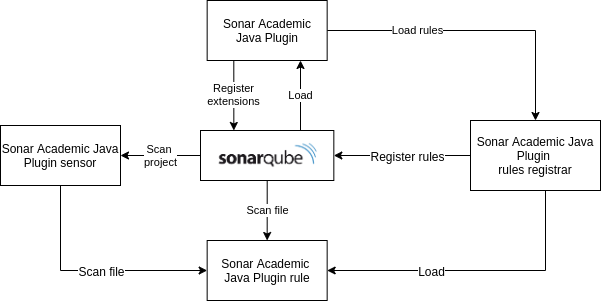
\includegraphics[scale=0.7]{figures/architecture_diagram.png}
        \caption{High level architecture of Sonar Academic Java Plugin.}
        \label{architecture_diagram}
    \end{center}
\end{figure}

The plugin is open source and full implementation can be found in the Github repository~\cite{sonar_plugin}.
The implementation contains not only the rules for the code smell detection, but also additional classes
that are required for the correct operation and rule registration inside SonarQube instance.

\FloatBarrier

\subsubsection{Translating queries into SonarQube rules}\label{subsubsec:translating-queries}

\TODO{
    Describe how queries from Kristiina's paper were transformed into SonarQube implementation.
}

As the code smells described by~\citeauthor{refactoring-fowler} are quite abstract, we needed
a more concrete definitions in order to implement the code smells.
In this paper, code smells are defined as Neo4j queries.
However, SonarQube uses different pattern for code smell detection.

In SonarQube, code smells are detected by applying visitor pattern~\cite{visitor_pattern} on the parsed
AST of Java source code.
Code smells are detecting by visiting specific nodes in the tree (such as classes or methods) and analyzing
the visited nodes in order to find the code smell pattern.
So in order to translate Neo4j queries into the definitions that are applicable to SonarQube, we used the following
algorithm that can be seen in~\ref{alg:translation_algorithm}.

Firstly, we needed to determine to context of the rule, such as if the rule should detect methods, classes or variables.
Then, we needed to decide if the rule required could be detected in a single scan of the context.
For example, if we need to decide whether or not the method has $X$ amount of parameters, we need would need to visit
this single method only a single time and we do not need to know anything about other methods.
But in some cases, we need to account for other nodes in the tree.
For example, in \verb|Shotgun Surgery| we need to detect method invocations that can be present in other classes.

\begin{algorithm} [!htb]
    \caption{Translation Neo4j queries into SonarQube rules}
    \label{alg:translation_algorithm}
    \KwIn{Neo4j query}
    \KwResult{Neo4j query translated into SonarQube implementation}
    \SetKwFunction{DetermineContext}{DetermineContext}
    \SetKwFunction{SensorRule}{SensorRule}
    \SetKwFunction{RegularRule}{RegularRule}
    \SetKwData{Context}{context}
    \SetKwData{q}{q}
    \SetKwData{r}{r}
    \BlankLine

    \ForEach{Neo4j query \q}{ \\
        \Context$\leftarrow$ \DetermineContext{$q$} \\
        \uIf{rule \r classes required for context $> 1$}{ \\
            \SensorRule{\Context, \r}; \\
        }
        \Else{ \\
            \RegularRule{\Context, \r}; \\
        };
    }
\end{algorithm}

As we can see from~\ref{alg:translation_algorithm}, there are 2 types of rules.
Regular rules (defined as \verb|RegularRule| in algorithm) require the context only of a single class under analysis.
Those are the rules, where we can decide whether a specific code smell exists or not just by looking at a single node
and its sub-nodes.
Example of such rules are \verb|Data class|, \verb|Message chains| or \verb|Blob class|.

However, for some rules, we need more than a context of a single file.
Examples of such rules are: \verb|Brain method| and \verb|Cyclic dependencies|.
In order to give more freedom to plugin writers, SonarQube provides an additional way to write custom rules - sensors.
\verb|Sensor| is an interface provided by SonarQube, which defines only a single method \verb|execute|.
This is called by the scanner during the analysis and the behaviour of this method is defined by the implementation.
So, we created own sensor that contains stateful rules.
The sensor accepts Java files, parses them into the AST, adds type information and then passes the AST to the rules.
Rules scan the tree passed by the sensor.
After all of the rules have been scanned, sensor calls method \verb|afterAllScanned|, indicating that all of the
input classes have been scanned and allows rules to report any issues detected during the analysis.
Visualization of the sensor analysis can be seen in algorithm~\ref{alg:sensor_algorithm}.

\begin{algorithm} [!htb]
    \caption{Performing analysis using sensor}
    \label{alg:sensor_algorithm}
    \KwIn{Sensor context}
    \KwResult{Analysis results reported to SonarQube server}
    \SetKwFunction{CreateClassPath}{CreateClassPath}
    \SetKwFunction{ParseJavaFile}{ParseJavaFile}
    \SetKwFunction{UpdateSymbolicModel}{UpdateSymbolicModel}
    \SetKwFunction{Scan}{Scan}
    \SetKwFunction{AfterAllScanned}{AfterAllScanned}
    \SetKwFunction{UploadResults}{UploadResults}
    \SetKwData{AST}{AST}
    \SetKwData{AstWithSymbolicModel}{AstWithSymbolicModel}
    \SetKwData{c}{c}
    \SetKwData{r}{r}
    \SetKwData{j}{j}
    \BlankLine

    \c$\leftarrow$ \CreateClassPath; \\

    \ForEach{Java file \j} {
        \AST$\leftarrow$ \ParseJavaFile { \j }; \\
        \AstWithSymbolicModel$\leftarrow$ \UpdateSymbolicModel{\j, \c};

        \ForEach{Rule \r} {
            \Scan{\r, \AstWithSymbolicModel};
        };
    }

    \ForEach{Rule \r} {
        \AfterAllScanned{};
    }

    \UploadResults{};
\end{algorithm}

\FloatBarrier

\subsubsection{Testing}

\TODO{
    Here describe that we did unit testing for each rule, and in the end achieved line coverage of 97\%
}

\TODO{
    Run the tests to see how many test cases we have.
}

As mentioned in~\ref{subsec:testing}, we also performed internal testing before applying tool to the real projects.
We performed unit testing using \verb|Scalatest|~\cite{scalatest}.
In order to measure line coverage, we used \verb|codecov|~\cite{codecov} which allowed us to measure
code coverage during every build in the continuous integration (CI) environment.

In the end, we had at least a single positive test case (a code pattern where our analyzer should detect a code smell)
for every rule that we have implemented and we achieved line coverage of $97.25\%$ with $92$ test cases.


    \subsection{Analysis results}\label{subsec:analysis-results}

    
\TODO{
    How many applications analyzed?
    How many lines (min, max avg)?
    Why others didnt get analyzed?
}

As the result, 193 applications were successfully analyzed.
This number is vastly different from the total amount of applications (1509) that are present in the corpus for multiple reasons.
Firstly, some of the projects were not using a build system (Gradle or Maven).
This is an issue because to compile the project we would need to specify the Classpath manually and
this is quite difficult to do programmatically.
Moreover, even if we managed to compile the projects, SonarQube is provided as a plugin for the build systems which means
that we would still not be able to run the analysis.
Secondly, some of the projects required extra configuration before building, which is also not possible to do
programmatically because each project is different and requires manual configuration.

The analysis was performed on a machine with \verb|Intel(R) Core(TM) i5-8250U CPU|\verb| @ 1.60GHz| and 16GB of RAM\@.
The statistics gathering for the thresholds took $441$ minutes in total with $2.24$ minutes on average per project.
However, running a project with all of the rules for code smell detections took $565$ minutes with $2.93$ minutes on average per project.
Note that this includes only the analysis itself and does not factor in the process of bulding and compiling the source
application.

In total, we analyzed $1450793$ lines of code.
On average, each application had $6843.363$ lines of code with a median of $2982$ lines of code.
The largest application contained $52358$ lines of code and the smallest application had $73$ lines of code.
The total number of detected code smells is $160775$ which means that there are $0.11$ code smells on average per line of code.

\TODO{
    Threshold gathering and calculation.
    Say the we collected thresholds two times, since first time we didn't exclude anonymous classes.
    Provide both tables with anonymous classes and without.
    Also show we calculated thresholds in the end.
    Say that for those that are missing we didnt have time and did gather them.
    We reused thresholds from Kristiinas' paper.
}

In section~\ref{subsec:analysis-procedure} we mentioned collecting the thresholds for some of the code smells.
The main idea for calculating the thresholds for the corpus is that this way we can reduce
the amount of false-positive detections and only detect the cases where the presence of the code smell is evident.

Table~\ref{threshold_calculation_table} shows the statistics that were used to calculate the thresholds for the
The first column shows the node type which was used to calculate the attribute.
The second columns displays the attribute name that was calculated for the specific node.
Columns $Q_1$, $Q_2$ and $Q_3$ display different quartiles for the collected values.

As mentioned in section~\ref{subsec:analysis-procedure}, the statistics were gathered from the analyzed applications.
In order to obtain the thresholds, we had to run the threshold collection 2 times, since during the first analysis
we did not exclude the anonymous classes.
We decided that anonymous classes should be excluded from the threshold collection since in Android applications
anonymous classes are used for listeners and thus occur very often because listeners are used in order to react to
user inputs and mobile applications are mostly about working with user input.

\begin{table}
    \begin{center}
        \begin{tabular} {| c | c | c | c | c |}
            \hline
            \textbf{Location} & \textbf{Event type} & \textbf{$Q_1$} & \textbf{$Q_2$} & \textbf{$Q_3$} \\ \hline
            Class & attributes & 1 & 2.0000000 & 5.000000 \\ \hline
            Class & cohesion & -1 & -1.0000000 & 0.000000  \\ \hline
            Class & comments & - & - & - \\ \hline
            Class & complexity & 0 & 3.0000000 & 12.500000 \\ \hline
            Class & complexityRatio & 0 & 0.8888889 & 2.467376 \\ \hline
            Class & coupling & - & - & - \\ \hline
            Class & instructions & 4 & 16.0000000 & 45.000000 \\ \hline
            Class & methods & 1 & 3.0000000 & 7.000000 \\ \hline
            Method & calls & - & - & - \\ \hline
            Method & chainLength & 2 & 2.0000000 & 3.000000 \\ \hline
            Method & complexity & 0 & 0.0000000 & 2.000000 \\ \hline
            Method & instructions & 1 & 2.0000000 & 8.000000 \\ \hline
            Method & parameters & 0 & 1.0000000 & 1.000000 \\ \hline
            Method & switchStatements & 0 & 0.0000000 & 0.000000 \\ \hline
            Interface & numberOfMethods & 1 & 1.0000000 & 2.000000 \\ \hline
        \end{tabular}
        \caption{\label{threshold_calculation_table}Values used for threshold calculation.}
    \end{center}
\end{table}

As it can be seen, some of the values are missing from the table~\ref{threshold_calculation_table}.
Due to time constraints, we were not able to collect all of the required statistics for all of the code smells
and since we were missing some of the values, we reused the values that were used by~\citeauthor{ios_code_smell_paper} in~\cite{ios_code_smell_paper}.

The complete list of calculated thresholds can be seen in table~\ref{threshold_values_table}.
Values written in \texttt{italics} were not calculated based on table~\ref{threshold_calculation_table} due to missing values
and thus were reused from the paper by~\cite{ios_code_smell_paper}.
This were the thresholds that were the used for code smell detection when retrieving the results.
The column \say{Code smell name} displays the rule for which the threshold was calculated.
The column \say{Variable} displays the variable for which the threshold was calculated in the rule.
The column \say{Mapping from threshold table} displays the \say{Location} and \say{Event type} from table~\ref{threshold_calculation_table}
that was used in order to calculate the value.
The column \say{Formula} shows the formula that was used to calculate teh value.
The column \say{Value} shows the final value that was used for \say{Variable} for the rule inside \say{Code smell name}.

\begin{landscape}
    \begin{table}
        \begin{center}
            \scalebox{0.9}{
                \begin{tabular} {| c | c | c | c | c |}
                    \hline
                    \textbf{Code smell name} & \textbf{Variable} & \textbf{Mapping from table~\ref{threshold_calculation_table}} & \textbf{Formula} & \textbf{Value} \\ \hline
                    Long method & veryHighNumberOfInstructions & Method: instructions & $Q_3 + (Q_3 - Q_1)*1.5$ & 18.5  \\ \hline
                    Blob class & veryHighLackOfCohesionInMethods & Class: cohesion & $Q_3 + (Q_3 - Q_1)*1.5$ & 1.5  \\ \hline
                    Blob class & veryHighNumberOfMethods & Class: methods & $Q_3 + (Q_3 - Q_1)*1.5$ & 16  \\ \hline
                    Blob class & veryHighNumberOfAttributes & Class: attributes & $Q_3 + (Q_3 - Q_1)*1.5$ & 11  \\ \hline
                    Shotgun surgery & veryHighNumberOfCallers & Method: calls & $Q_3 + (Q_3 - Q_1)*1.5$ & \texttt{2.5}  \\ \hline
                    Switch statements & veryHighNumberOfSwitchStatements & Method: switchStatements & $Q_3 + (Q_3 - Q_1)*1.5$ & 0  \\ \hline
                    Lazy class & mediumNumberOfInstructions & Class: instructions & $Q_2$ & 16  \\ \hline
                    Lazy class & mediumCouplingBetweenObjectClasses & Class: coupling & $Q_2$ & \texttt{0}  \\ \hline
                    Message chains & veryHighNumberOfChainedMessages & Method: chainLength & $Q_3 + (Q_3 - Q_1)*1.5$ & 4.5  \\ \hline
                    Comments & veryHighNumberOfComments & Class: comments & $Q_3 + (Q_3 - Q_1)*1.5$ & \texttt{29.5}  \\ \hline
                    Divergent change & veryHighNumberOfCalledMethods & - & $Q_3 + (Q_3 - Q_1)*1.5$ & \texttt{2.5}  \\ \hline
                    Long parameter list & veryHighNumberOfParameters & Method: parameters & $Q_3 + (Q_3 - Q_1)*1.5$ & 2.5  \\ \hline
                    Middle man & lowNumberOfInstructionsMethod & Method: instructions & $\max(Q_1 - (Q_3 - Q_1)*1.5, 0)$ & 0  \\ \hline
                    Inappropriate intimacy & highNumberOfCallsBetweenClasses & - & $Q_3$ & \texttt{5}  \\ \hline
                    Brain method & highNumberOfInstructionsForClass & Class: instructions & $Q_3$ & 45  \\ \hline
                    Brain method & highCyclomaticComplexity & Method: complexity & $Q_3$ & 2  \\ \hline
                    God class & veryHighWeightedMethodCount & Class: complexity & $Q_3 + (Q_3 - Q_1)*1.5$ & 6.16844  \\ \hline
                    Primitive obsession & veryHighPrimitiveVariableUse & - & Q_3 + $(Q_3 - Q_1)*1.5$ & \texttt{6}  \\ \hline
                    Complex class & veryHighClassComplexity & Class: complexity & $Q_3 + (Q_3 - Q_1)*1.5$ & 31.25  \\ \hline
                    Swiss army knife & veryHighNumberOfMethods & Interface: numberOfMethods & $Q_3 + (Q_3 - Q_1)*1.5$ & 3.5 \\ \hline
                \end{tabular}
            }
            \caption{\label{threshold_values_table}Calculated thresholds based on values from table~\ref{threshold_calculation_table}.}
        \end{center}
    \end{table}
\end{landscape}

\TODO{
    Show results.
    How many applications contained code smell X?
    How do those code smells distribute inside analyzed applications?
}

\TODO{
    Need more input here.
    What should I include here?
}

Now that we have shown the general information about the analysis process and thresholds, we can finally go over
the results that we found.
Figure~\ref{fig:applicaitons_contain_x} shows the how many of the applications actually contain each code smell.

\begin{figure}
    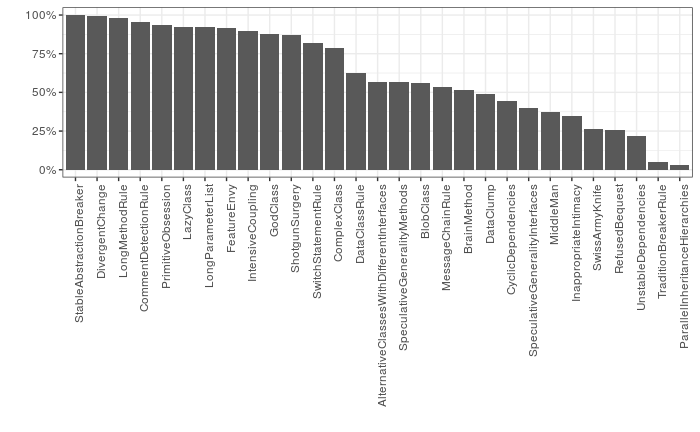
\includegraphics[scale=0.8]{figures/applications_contains_x_2.png}
    \caption{How many applications contain code smell $X$?}
    \label{fig:applicaitons_contain_x}
\end{figure}

As one can see, there is a high number of code smells that are present in over $75\%$ of the applications.

Figure~\ref{fig:distribution}, shows distribution of detected code smells inside analyzed applications.

\begin{figure}
    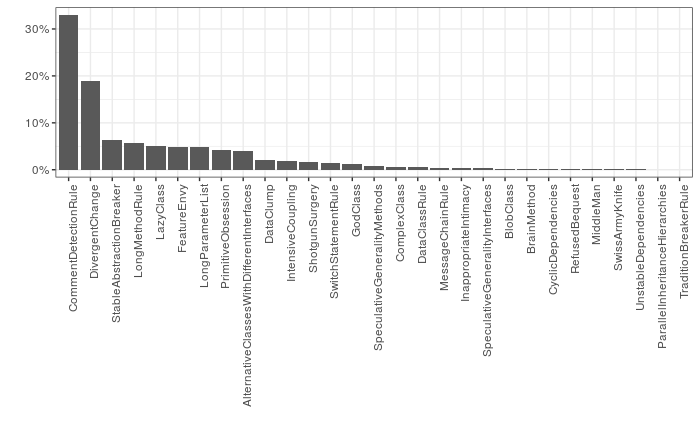
\includegraphics[scale=0.8]{figures/distribution_2.png}
    \caption{Distribution of code smells inside the analyzed applications.}
    \label{fig:distribution}
\end{figure}

\FloatBarrier

\TODO{
    Comments make up a big part of distribution.
    Perhaps we should make a separate figure without comments included?
}



    \newpage
    \section{Discussion}\label{sec:discussion}

    \subsection{Encountered problems}\label{subsec:encountered-problems}

In this section, we will discuss the difficulties encountered during the development of the plugin.

The first problem is related to the analysis model of the SonarQube.
Currently, SonarQube assumes that all the code smells can be detected during a single
analysis of an AST node.
The issue is that a large number of code smells implemented by us require the context of other AST nodes.
For example, to find cyclic dependencies, we first need to detect all the dependencies
of a class and then, after all the dependencies of all the classes inside of the application have been detected,
we would transform the dependencies into a graph and look for the cycles in the graph.

Fortunately, SonarQube provides a possibility to implement sensors, which can fully control the execution flow
of the analysis.
By using sensors, we were able to create a custom execution pipeline for the rules that require the context of the project
and not just a single node.
This approach allowed us to solve the original problem, but lead to another one.

The second problem is related to the API that SonarQube plugin base exposes.
As mentioned in section~\ref{subsec:sonarqube-plugin-development}, we followed the guide provided by the SonarQube community to implement our plugin.
This includes the usage of the base dependency which includes the API for accessing the AST generated by SonarQube.
Additionally, this dependency also contains other utilities, such as various visitors which can be used to detect
various measures inside the code such as complexity or count the lines of code.
The problem is that some classes are available only during the compilation phase of the application and
are missing from the runtime environment when the plugin is loaded for the analysis execution.

As mentioned previously, we used sensors to implement the pipeline for the rules that have state.
The sensor pipeline has to be built from scratch as the input that you receive are source files of the project and not
parsed AST as it is with normal rules.
This means that we needed to parse the files into the AST by ourselves, and it was not that simple to do due to some
classes missing from the runtime.

One of the solutions could be to include the full library inside the compiled artifact and bring all those classes with
the plugin itself.
This would mean we would also bring the implementations of the AST tree nodes and this would cause
\verb|ClassCastException|-s at runtime of the plugin because of how Java Virtual Machine (JVM) handles classes loaded
by different class loaders: even though the classes are effectively the same if they were loaded by the different class loaders
JVM cannot guarantee that they are indeed the same, so casting between those types is not allowed.

To fix this issue, we forked the plugin base dependency and all the classes
that are exposed by the API were left out of it, to fix the aforementioned problem with class loaders.
Then we could use our dependency to parse the input files to AST the same way SonarQube would do it
and use all the utilities that are present in the SonarQube base dependency for our own needs.

The library is also open source and can be found in the Github repository~\cite{sonar_java_extracted}.

\subsection{Issues and limitations}\label{subsec:issues-and-limitations}

After the implementation has been completed, there are still some issues that we would like to fix in the future.

Firstly, some rules have been implemented as normal SonarQube rules, when they should be implemented as sensor rules.
As an example, let us look into \verb|Shotgun surgery|.
This rule was implemented as a regular SonarQube rule although it has state and this results in a situation where
we have to check for issues after every scanned class because we never know whether this class is the last we would scan.
This was implemented so because the implementation of the rule was done before we developed the internal sensor \say{framework},
and there was no reason to rewrite it because it works the way it is implemented now.
Nonetheless, it would be more efficient to rewrite this rule as a sensor rule.

Secondly, we did not have time to implement nice descriptions of the rules.
SonarQube UI provides a possibility to include a description for the rule that the user would read to understand the idea behind the rule and also see compliant / non-compliant code examples as it can be seen
in figure~\ref{fig:sonarqube_description_example}.
Additionally, on that page, we can see the type of the detection (which in our case is \say{Code smell}) and
the severity of the detection, which is set by the user when activating the rule for the specific case (which is set to \say{minor} by default for our rules).

\begin{figure}
    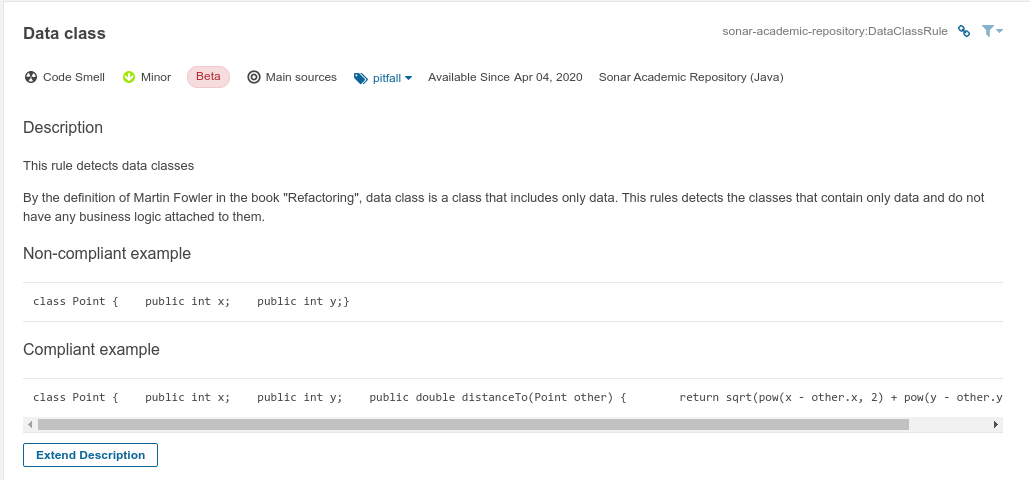
\includegraphics[scale=0.45]{figures/sonarqube_description.png}
    \caption{SonarQube rule description example.}
    \label{fig:sonarqube_description_example}
\end{figure}

Currently, we assume that the user is familiar with the rules and does not require any assistance in understanding how
a given rule works, but it would still be nice to have complete and concise descriptions about rule implementations.

Finally, there as an issue with threshold calculation that has been mentioned in section~\ref{subsec:analysis-results}.
As we did not calculate some thresholds by ourselves, they might be drastically different for Java applications from
Swift applications.

\FloatBarrier

\subsection{Comparison to published results}\label{subsec:comparison-to-published-results}

In section~\ref{sec:results} we introduced the results that we collected when analyzing our corpus
of the applications.
Previously, \citeauthor{mannan2016understanding} in~\cite{mannan2016understanding} also investigated code smells in
Android applications.
The main reason why we want to compare the tool described in this paper to the tool used in~\cite{mannan2016understanding}
is that the tool used in that paper is no longer available.
As it was closed-source, commercial solution for code smell analysis, we would like to know how our implementation
compares to the one in~\cite{mannan2016understanding}.

As~\citeauthor{mannan2016understanding} did not provide any concrete distribution of the detected
code smells inside analyzed applications, we had to rely on figure 2 in~\cite{mannan2016understanding} in order
to get the values collected as a result of the analysis.
Table~\ref{tab:understading_andoid_smells_values} shows the values that we were able to extract from the figure which we used for comparison
with our results.
The figure contains two datasets (\say{mobile} and \say{desktop} applications) and we used the values for the \say{mobile}
dataset, since we were analyzing applications for the Android platform.

\begin{table}
    \begin{center}
        \begin{tabular} {| c | c |}
            \hline
            \textbf{Code smell name} & \textbf{Percentage of occurrence (\%)} \\ \hline
            Data class & 18 \\ \hline
            Data clump & 15.5 \\ \hline
            Cyclic dependencies & 13 \\ \hline
            Feature envy & 9.5 \\ \hline
            External duplication & 9 \\ \hline
            SAPBreaker & 9 \\ \hline
            God class & 5.5 \\ \hline
            Sibling duplication & 4.5 \\ \hline
            Divergent change & 4 \\ \hline
            Message chains & 2.5 \\ \hline
            Intensive coupling & 2.4 \\ \hline
            Tradition breaker & 2 \\ \hline
            Unstable dependencies & 1.75 \\ \hline
            Refused bequest & 1.5 \\ \hline
            Blob class & 1 \\ \hline
            Shotgun surgery & 0.5 \\ \hline
            Internal duplication & 0.25 \\ \hline
        \end{tabular}
        \caption{Distribution of detected code smells from~\cite{mannan2016understanding}.}
        \label{tab:understading_andoid_smells_values}
    \end{center}
\end{table}

As in our paper, we analyzed more than the code smells than in~\cite{mannan2016understanding}, we had to normalize
our results so that we could compare the distribution only of those code smells that are present in~\cite{mannan2016understanding}.
Table~\ref{tab:sonar_academic_plugin_values} shows normalized distribution of the code smells (only the ones that
are present in~\cite{mannan2016understanding}).

\begin{table}
    \begin{center}
        \begin{tabular} {| c | c |}
            \hline
            \textbf{Code smell name} & \textbf{Percentage of the occurrence (\%)} \\ \hline
            Data class & 14.7854994 \\ \hline
            Data clump & 5.32531265 \\ \hline
            Cyclic dependencies & 0.54297926 \\ \hline
            Feature envy & 12.69273389 \\ \hline
            SAPBreaker & 16.37011240 \\ \hline
            God class & 3.07424410 \\ \hline
            Divergent change & 48.62751306 \\ \hline
            Message chains & 1.24267849 \\ \hline
            Intensive coupling & 5.06252968 \\ \hline
            Tradition breaker & 0.02691151 \\ \hline
            Unstable dependencies & 0.17255026 \\ \hline
            Refused bequest & 0.50498654 \\ \hline
            Blob class & 0.66170651 \\ \hline
            Shotgun surgery & 4.21719171 \\ \hline
        \end{tabular}
        \caption{Distribution of selected code smells for this paper.}
        \label{tab:sonar_academic_plugin_values}
    \end{center}
\end{table}

A comparison of distributions of both papers can be seen in figure~\ref{fig:comparison_of_distributions}.
It is important to note that we left some of the code smells out of the comparison.
The reason is that we did not implement those rules in our plugin, as those are already natively
supported by SonarQube.
The rules that we excluded from the comparison are \say{external duplication}, \say{sibling duplication} and
\say{internal duplication}.


From this comparison, we can see that the number of detections for some code smells is pretty similar and quite different for others.
For instance, the number of detections for \say{blob class} and \say{feature envy} is pretty similar, while
\say{data class} and \say{divergent change} are quite different.

There are multiple reasons why the results are different but here are the ideas on why the difference more noticeable in
some occasions than others.

\begin{flushleft}
    \textbf{Implementation might be different}.
    This means that the code smell definitions in~\cite{mannan2016understanding} might be different from our definition and thus we are detecting different things or detecting the same things differently.
    Since the tool from~\cite{mannan2016understanding} is closed-source then we are not able to compare the implementations.
\end{flushleft}

\begin{flushleft}
    \textbf{Corpuses are different}.
    The source datasets were not provided by~\citeauthor{mannan2016understanding}, so we are not able to verify our tool against the same dataset.
    If we used the same dataset, the results might have been more similar or, on the contrary, different.
\end{flushleft}

\begin{figure} [htb]
    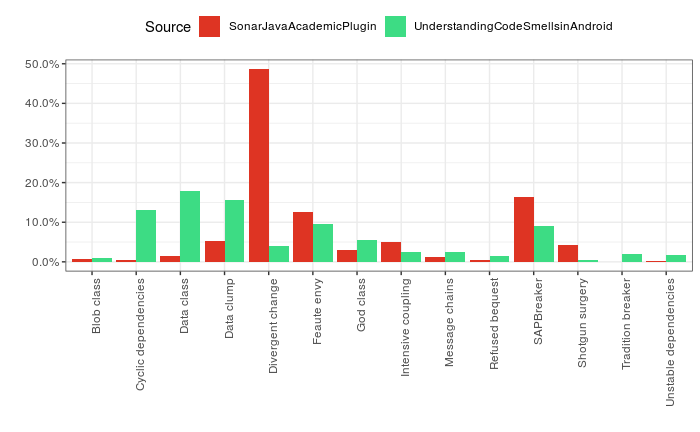
\includegraphics[scale=0.8]{figures/comparison_2.png}
    \caption{Distribution of detected code smells in our paper versus~\cite{mannan2016understanding}.}
    \label{fig:comparison_of_distributions}
\end{figure}

As the reader might have noticed, there are various reasons why the results might be different.
Nonetheless, different results on different datasets do not mean that one tool is more useful than the other.
In the next chapter, we will look into the potential usages of the tool developed by us.

\FloatBarrier

\subsection{Potential usages}\label{subsec:potential-usages}

In section~\ref{sec:introduction} we mentioned various roles in software development process who might be interested
in the results of an analysis of a software project.
In the next subsections, we will go over the ways how each of the focus groups can use the plugin.

\subsubsection{Developers}

Developers are our main target group.
SonarQube also can be integrated into the IDE and be used from there.
Unfortunately, this requires the premium edition (paid) of SonarQube and we only have access to the community edition (free)
so we are not able to show the screenshots from the IDE\@.
Nonetheless, full information is available on the server-side after the analysis has been run in the CI/CD environment.
Figure~\ref{fig:dev_1} shows the information that the developer sees when a code smell is reported on the Sonar server side.
In the picture we can see the message that was reported by the static analyzer, when it was first introduced,
the line it occurs on, what is the type of reported issue (in our case it is \say{code smell}) and severity of the detection.

\begin{figure}
    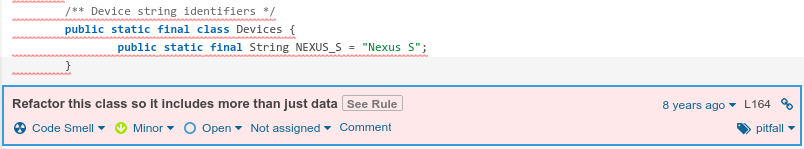
\includegraphics[scale=0.5]{figures/dev_1.png}
    \caption{Example of a reported issue on the server side.}
    \label{fig:dev_1}
\end{figure}

Additionally, the developer has an option to press the \say{See rule} button.
When opened, this view shows the description of the reported code smell, as it can be seen in figure~\ref{fig:dev_2}.
This allows the developers to quickly access rule definitions to see compliant and non-compliant rule examples.

\begin{figure}
    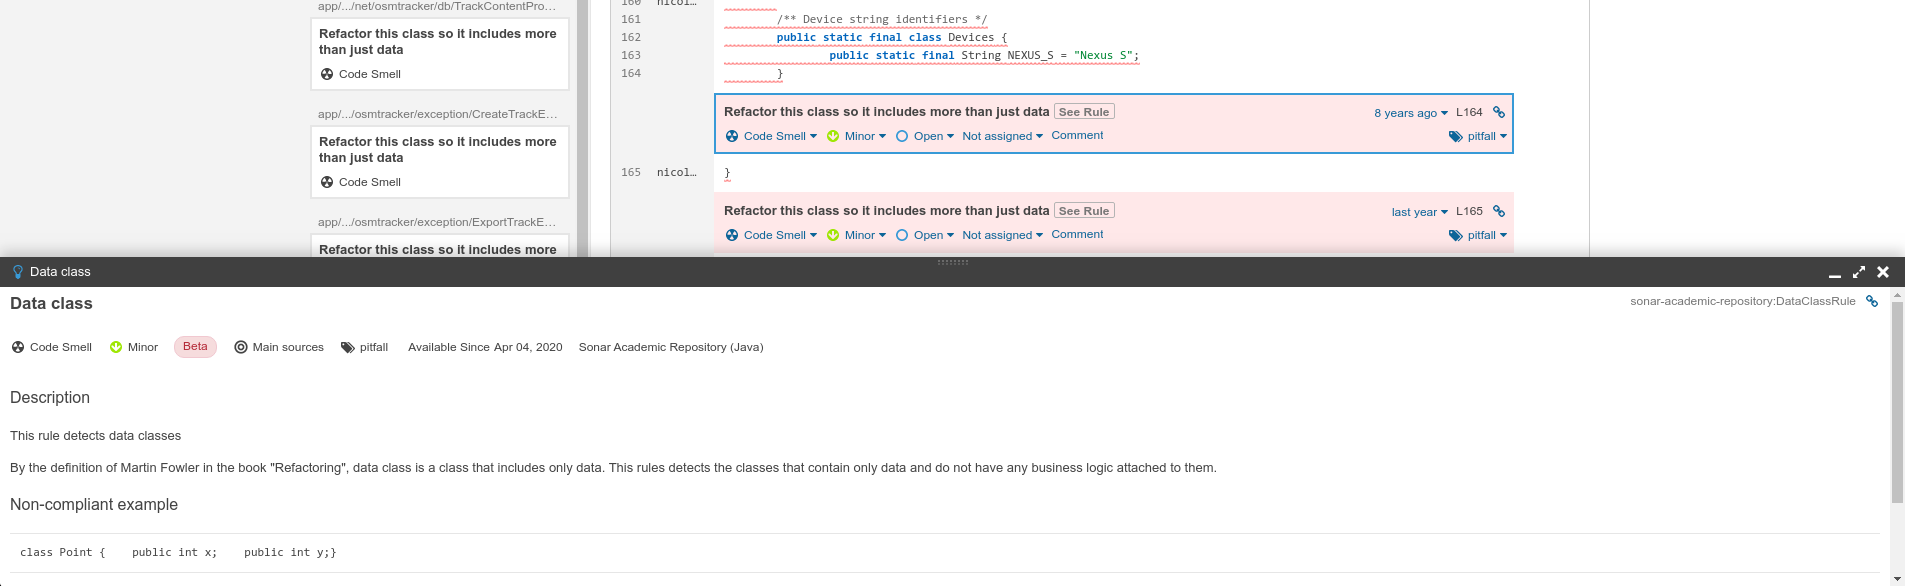
\includegraphics[scale=0.25]{figures/dev_2.png}
    \caption{Example of expanded rule description.}
    \label{fig:dev_2}
\end{figure}

\FloatBarrier

\subsubsection{Project managers}

As mentioned in the previous section, it is possible to integrate the plugin into the IDE.
However, not all the roles in software development are related to coding.
SonarQube provides a nice user interface, that can be useful for project managers to receive an overview of a project,
as seen in figure~\ref{fig:spm_1}.
In this figure, we can see different metrics that are helpful to identify the state of the project.
For example, the number of bugs, vulnerabilities, and code smells detected during static code analysis.

\begin{figure}
    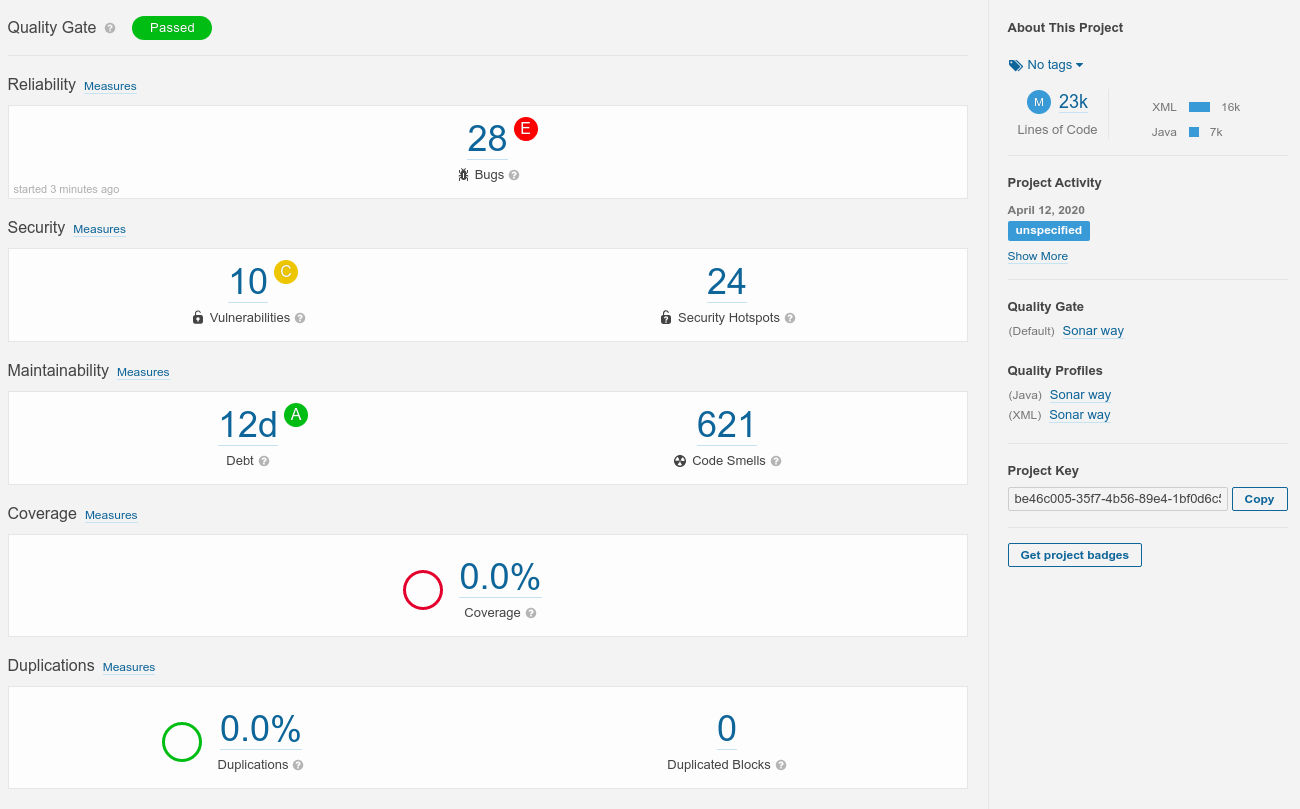
\includegraphics[scale=0.35]{figures/project_managers_1.png}
    \caption{Example of a project overview in the SonarQube user interface.}
    \label{fig:spm_1}
\end{figure}

The view of figure~\ref{fig:spm_1} can be further expanded to see a more detailed overview of detected
code smells/vulnerabilities as can be seen in figure~\ref{fig:spm_2}.

\begin{figure}
    \centering
    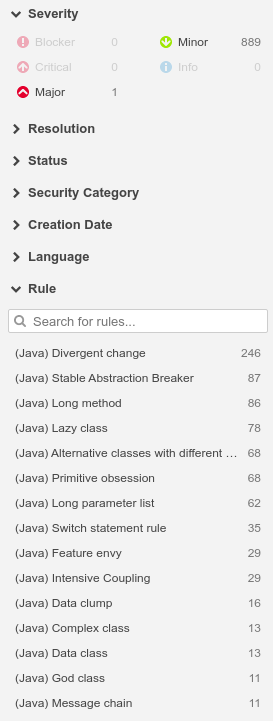
\includegraphics[scale=0.6]{figures/pm_2_1.png}
    \caption{Example of code smell detections grouped by rule.}
    \label{fig:spm_2}
\end{figure}

\FloatBarrier

\subsubsection{Data scientists}

In the era of big data, a lot of useful information can be extracted from the collected data.
Static code analysis is not an exception.
If an organization maintains multiple projects in a SonarQube instance, the data from the static
analysis could be used to find correlations between different code smells in multiple projects.
This could show some trends where certain code smells are popular in multiple teams and could
lead to the introduction of new rules to fix the code quality issues.

SonarQube provides a rich set of web services that can be used to extract the data into external applications.
The base URI \url{/api/webservices/list} describes all web services exposed by the current SonarQube instance.
For example, the API can be used to export the issues found in the project for further analysis.
To achieve this, one would use the \url{/api/issues/search} endpoint to search for issues inside the projects.


    \newpage

    \section{Conclusion}\label{sec:conclusion}

    \TODO{
        Say that we have created a tool and it works on the projects that we checked,
        but we dont know if it actually helps, since we did not perform any empirical study.
        Say that there might be some limitations with the dataset that we have selected.
        Discuss future work.
    }

% BibTeX bibliography
    \newpage
    \bibliographystyle{plainnat}
    \bibliography{masters-thesis-template}

    \addcontentsline{toc}{section}{\refname}


% Use Biblatex if you have problems with Estonian keywords
%\printbibliography %biblatex



    \newpage
%\appendix
%\section*{\appendixname}
    \iflanguage{english}%
    {\section*{Appendix}
        \addcontentsline{toc}{section}{Appendix}
    }%
    {\section*{Lisad}
        \addcontentsline{toc}{section}{Lisad}}


    \section*{I. Glossary}
    \addcontentsline{toc}{subsection}{I. Glossary}

    \newpage

%=== Licence in English
    \newcommand{\licencehint}[2]{\\\hspace*{#1}\textsl(#2)\par}
    \newcommand\EngLicence{{%
        \selectlanguage{english}
        \section*{II. Licence}

        \addcontentsline{toc}{subsection}{II. Licence}

        \subsection*{Non-exclusive licence to reproduce thesis and make thesis public}

        I, \textbf{Stanislav Mõškovski}, %author's name
        \licencehint{10mm}{author's name}

        \begin{enumerate}
            \item
            herewith grant the University of Tartu a free permit (non-exclusive licence) to
            \par
            reproduce, for the purpose of preservation, including for adding to the DSpace digital archives until the expiry of the term of copyright,
            \par
            \textbf{Building a tool for detecting code smells in Android application code}, %
            \licencehint{10mm}{title of thesis}
            \par
            supervised by Kristiina Rahkema and Dietmar Pfahl. %supervisor's name
            \licencehint{10mm}{supervisor's name}
            \item
            I grant the University of Tartu a permit to make the work specified in p. 1 available to the public via the web environment of the University of Tartu, including via the DSpace digital archives, under the Creative Commons licence CC BY NC ND 3.0, which allows, by giving appropriate credit to the author, to reproduce, distribute the work and communicate it to the public, and prohibits the creation of derivative works and any commercial use of the work until the expiry of the term of copyright.
            \item
            I am aware of the fact that the author retains the rights specified in p. 1 and 2.
            \item
            I certify that granting the non-exclusive licence does not infringe other persons' intellectual property rights or rights arising from the personal data protection legislation.
        \end{enumerate}

        \noindent
        Stanislav Mõškovski\\ %author's name
        \textbf{\textsl{dd/mm/yyyy}}
    }}%\newcommand\EngLicence


%=== Licence in Estonian
    \newcommand\EstLicence{{%
        \selectlanguage{estonian}
        \section*{II. Litsents}

        \addcontentsline{toc}{subsection}{II. Litsents}

        \subsection*{Lihtlitsents lõputöö reprodutseerimiseks ja üldsusele kättesaadavaks tegemiseks}

        Mina, \textbf{Alice Cooper}, %author's name
        \licencehint{10mm}{autori nimi}

        \begin{enumerate}
            \item
            annan Tartu Ülikoolile tasuta loa (lihtlitsentsi) minu loodud teose
            \par
            \textbf{Tüübituletus neljandat järku loogikavalemitele}, %title of thesis
            \licencehint{10mm}{lõputöö pealkiri}
            \par
            mille juhendaja(d) on Axel Rose ja May Flower, %supervisor's name(s)
            \licencehint{10mm}{juhendaja nimi}
            \par
            reprodutseerimiseks eesmärgiga seda säilitada, sealhulgas lisada digitaalarhiivi DSpace kuni autoriõiguse kehtivuse lõppemiseni.
            \par
            \item
            Annan Tartu Ülikoolile loa teha punktis 1 nimetatud teos üldsusele kättesaadavaks Tartu Ülikooli veebikeskkonna, sealhulgas digitaalarhiivi DSpace kaudu Creative Commonsi litsentsiga CC BY NC ND 3.0, mis lubab autorile viidates teost reprodutseerida, levitada ja üldsusele suunata ning keelab luua tuletatud teost ja kasutada teost ärieesmärgil, kuni autoriõiguse kehtivuse lõppemiseni.
            \item
            Olen teadlik, et punktides 1 ja 2 nimetatud õigused jäävad alles ka autorile.
            \item
            Kinnitan, et lihtlitsentsi andmisega ei riku ma teiste isikute intellektuaalomandi ega isikuandmete kaitse õigusaktidest tulenevaid õigusi.
        \end{enumerate}

        \noindent
        Alice Cooper\\ %author's name
        \textbf{\textsl{pp.kk.aaaa}}
    }}%\newcommand\EstLicence


%===Choose the licence in active language
    \iflanguage{english}{\EngLicence}{\EstLicence}


\end{document}

